\chapter{Efficient knockoffs construction}\label{ch:sdp}

As shown in Chapter~\ref{ch:fs}, in the case of gaussian knockoffs
$\tX$ can be sampled from a normal distribution $\cN\left( \bupsilon,\, \Upsilon \right)$ whose parameters
$\bupsilon,\, \Upsilon$ are formulated in~\ref{eq:conditional_gaussian_knockoffs2}.
\begin{equation}\label{eq:conditional_gaussian_knockoffs2}
    \tcX \mid \cX \sim \cN\left( \bupsilon, \Upsilon \right)
    ,\qquad\text{where}\quad
    \begin{cases*}
        \bupsilon = \cX - \cX\Sigma^{-1}\diag(\bs)\\
        \Upsilon = \diag(\bs)\left( 2I_{p \times p} - \Sigma^{-1}\diag(\bs) \right)
    \end{cases*}
\end{equation}
More generally, the same parameters are derived by only imposing
$\big[ X, \tX \big]_{\swap\left( S \right)}$ and $\big[ X, \tX \big]$
to have equal first two moments
for any subset
$S \subseteq \left\{ 1, \dots, p \right\}$,
rather than the same distribution.
These formulas are valid for any vector $\bs \in \R^p$ such that $\Omega$
is indeed a covariance matrix (semidefinite positive).
\begin{equation*}
    \Omega = \begin{bmatrix}
        \Sigma & \Sigma - \diag \bs\\
        \Sigma - \diag \bs & \Sigma
    \end{bmatrix}
    \succeq \0_{2p \times 2p}
\end{equation*}
As shown in proposition~\ref{prop:omega_psd},
this matrix is semidefinite positive if and only if $\0_{p \times p} \preceq \diag \bs \preceq 2 \Sigma$.
The first inequality clearly holds if all the entries of $\bs$ are positive.
It is however trickier to identify all vectors $\bs$ satisfying the second one.

In this chapter, we show why the choice of $\bs$ is important and how to efficiently find a good one
in the high dimensional setting.
In the remaining, we note $\Sigma$ the true covariance and $\hat{\Sigma}$ its estimation from the samples $X$
(be it empirical or derived from more sophisticated methods).

\section{Equi-correlated knockoffs}\label{sec:equi}

\subsubsection{A cheap solution}

For any psd matrix $A \in \R^p$, $A + \alpha I_{p \times p}$ has the same eigenvalues as $A$, but shifted by $\alpha$.
It gives a fast and simple way to find a feasible $\bs$.
\begin{equation}\label{eq:equi}
    s_j = 2\lambda_{\min}(\cove)
    \quad\text{ for all } 0 \leq j \leq p
\end{equation}
The problem of finding the smallest eigenvalue $\lambda_{\min}(\cove)$ can be solved efficiently,
using for instance a singular value decomposition which runs in $\cO(p^3)$ steps~\cite{svd}.

\subsubsection{Why it is not desirable}

For large values of $p$,
the minimum eigenvalue of $\cove$ is likely to be very small,
unless $\cove$ has a substantially special structure.
Let us analyze briefly the covariance of $\big[ \cX; \tcX \big]$
to understand why it is unprofitable for the selection procedure.
If $\tcX$ is built according to~\ref{eq:conditional_gaussian_knockoffs2}, it satisfies
\begin{equation*}
    \begin{cases}
        \cov(\tcX_j,\, \tcX_{j'}) = \cov(\cX_j,\, \cX_{j'}) \text{ for all } j,\,j'\\
        \cov(\cX_j,\, \tcX_{j'}) = \cov(\cX_j,\, \cX_{j'}) \text{ for all } j \neq j'\\
        \cov(\cX_j,\, \tcX_j) = \cov(\cX_j,\, \cX_j) - s_j \text{ for all } j
    \end{cases}
\end{equation*}
First, $\tcX$ has the same internal covariance has $\cX$,
and two distinct original and knockoff features have the same covariance
as the one of the two corresponding original features.
It makes the knockoff features sufficiently close to the original features
to fool the estimator computing the statistics.
However, an original feature $j$ and its corresponding knockoff have a covariance that is smaller the larger $s_j$ is.
If $s_j$ is close to $0$,
$\cX_j$ cannot be distinguished from $\tcX_j$ and the selection would suffer from a low power.

This fact is even more detrimental when $p$ is large as $\lambda_{\min}$ is likely to be very close to $0$.
It motivates us to maximize the sum of the entries of $\bs$ and it leads to solving a SDP\@.

\section{SDP knockoffs}\label{sec:sdp}

This observation motivates us to maximize the entries of $\bs$,
while maintaining the inequality $\diag\bs \preceq \tcovm$.
This can be formulated in the optimization problem~\ref{eq:sdp}.
\begin{equation}\label{eq:sdp}
    \underset{\bs \in \R^p}{\argmax}\;\,
    \sum_{j = 1}^p s_j
    \qquad
    \text{subject to } \begin{cases}
        s_j \geq 0\text{ for all } j\\
        \diag \bs \preceq \tcove
    \end{cases}
\end{equation}
This problem is a structured semidefinite program (SDP) and can efficiently be solved for small values of
$p$ by interior point methods~\cite{interior_point_method_sdp} for example.
For larger values of $p$, even first order methods like
SCS~\cite{sdp_scs} or alternating direction~\cite{sdp_admm}
quickly become intractable.
In memory, it needs roughly $\cO(m^2)$ where $m$ is the number of constraints.
Even though the convergence speed depends a lot on $\cove$,
it experimentally appears that alternative methods have to be considered when $p > 1000$.
The Figure~\ref{fig:cvx_sdp_times} shows the convergence time of the solvers SCS and MOSEK as a function of $p$.
Theoretically, it takes $\cO(p^3)$ and it is clear that when $p$ is more than a few thousands.
Moreover, most solutions returned by these algorithms are actually infeasible because of numerical approximations.

\begin{figure}
    \centering
    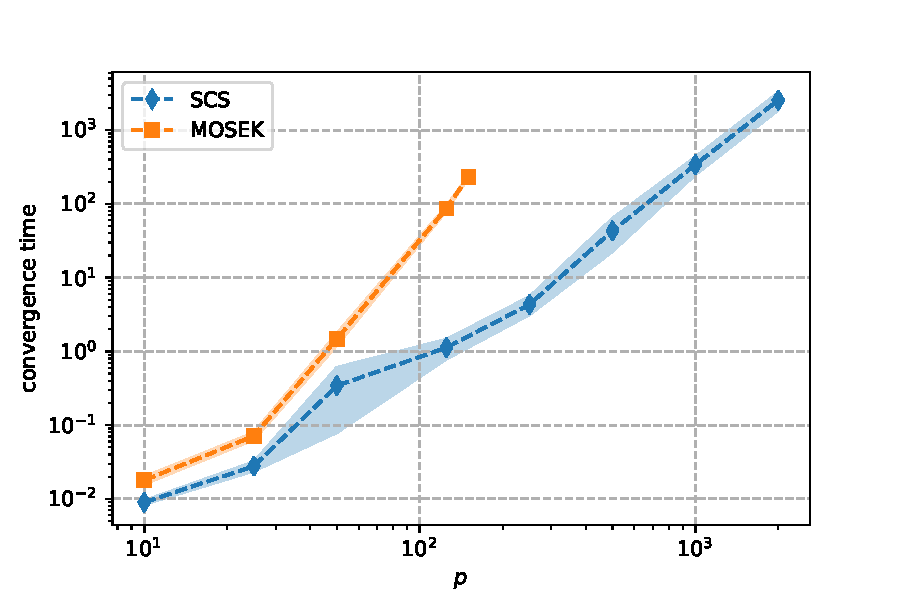
\includegraphics[width=0.8\linewidth, height=0.5\linewidth]{figures/cvx_sdp_times.pdf}
    \caption{
        Time (in seconds) required to converge for SCS (blue) and MOSEK (orange) solvers
        as a function of $p$ in log-log scale.
        Rapidly, MOSEK needs too much memory and can't be run for $p > 150$.
        Both match the theoretical $\cO(p^3)$ rate and SCS already needs 15 minutes for $p = 1000$.
        See Appendix~\ref{sec:cvx_times} for details regarding the random generation of covariance
        matrices $\cove$.
    }
    \label{fig:cvx_sdp_times}
\end{figure}

In order to reduce the computation time,
Barber-Candès suggest to solve an approximated problem of~\ref{eq:sdp} in 2 steps that we describe below.
\paragraph*{Step 1.}
Pick an approximation $\coveapprox$ of $\cove$ and solve
\begin{equation}\label{eq:sdp_approx}
    \underset{\hat{\bs} \in \R^p}{\argmax}\;\,
    \sum_{j = 1}^p \hat{s}_j
    \qquad
    \text{subject to } \begin{cases}
        \hat{s}_j \geq 0\text{ for all } j\\
        \diag \hat{\bs} \preceq \tcoveapprox
    \end{cases}
\end{equation}
\paragraph*{Step 2.}
Solve the one dimensional maximization
\begin{equation}\label{eq:sdp_approx_1d}
    \underset{\gamma \in \R}{\argmax}\;\,\gamma
    \quad\text{subject to}\quad
    \diag\left( \gamma \cdot \hat{\bs} \right) \preceq \tcove
\end{equation}
Finally, pick $\bs = \gamma \cdot \hat{\bs}$.

\begin{remark}
    Note that the two extreme options $\coveapprox = \mI$ and $\coveapprox = \cove$ yield
    the same solutions as solving equi-knockoffs~\ref{eq:equi} and full SDP knockoffs~\ref{eq:sdp} respectively.
\end{remark}

Solving~\ref{eq:sdp_approx_1d} in step 2 can be done very efficiently using bisection as it is a one-dimensional SDP\@.
The optimization problem~\ref{eq:sdp_approx} is however the same as the one in~\ref{eq:sdp},
except for the approximation $\coveapprox$.
To speed up the computations,
$\coveapprox$ can be chosen to be a block-diagonal matrix of $k$ blocks.
The maximization then reduces to $k$ smaller SDPs for which the solutions can be found more efficiently.
These could even be distributed in several computation nodes.
Picking $\coveapprox$ is a compromise between available computation time and eventual power of the procedure.
There is a priori no ideal way to to it.
The block diagonal assumption depends on the order of the features.
They should therefore be reordered ahead of time,
typically by performing a clustering step to group very similar features.

\section{A coordinate ascent approach}\label{sec:coordinate_ascent}

\subsection{Notations and preliminaries}\label{subsec:notations_preliminaries}

\paragraph{Notations.}
Let $M \in \R^{p \times p}$.
Given two sets of indices $\cI,\,\cJ \in \fset$,
we note $M_{\cI,\,\cJ}$ the $\abs{\cI} \times \abs{\cJ}$ matrix obtained by keeping
the $\abs{\cI}$ rows and $\abs{\cJ}$ columns indexed by $\cI$ and $\cJ$ respectively.
By convenience, an integer $j$ denotes the set $\left\{ j \right\}$ and $j^c$ $\fset \setminus \left\{ j \right\}$
in the matrix subscripting context.
For example, if $M = \begin{bmatrix}
    1 & 2 & 3\\
    4 & 5 & 6\\
    7 & 8 & 9
\end{bmatrix}$,
then $M_{1^c, 1^c} = \begin{bmatrix}
    5 & 6\\
    8 & 9
\end{bmatrix}$
and $M_{1^c, 1} = \begin{bmatrix}
    4\\
    7
\end{bmatrix}$.

\paragraph{Positiveness characterisation.}
Suppose $M$ is structured as
\begin{equation*}
    M = \begin{bmatrix}
        \xi & \yy^\top\\
        \yy & B
    \end{bmatrix}
\end{equation*}
where $B$ is symmetric and invertible.
\begin{lemma}\label{lemma:schur1}
    Using Schur complements (see Appendix~\ref{sec:schur_complement}), it holds that M is psd if and only if
    \begin{equation*}
        B \succeq \0
        \quad\text{and}\quad
        \xi - \yy^\top B^{-1} \yy \geq 0
    \end{equation*}
\end{lemma}
In subscript notations, this is equivalent to $M_{1^c,\, 1^c} \succeq \0$ and
$M_{1,\, 1} - M_{1^c,\, 1}^\top M_{1^c,\, 1^c} M_{1^c,\, 1} \geq 0$.
This statement can be generalized as follows.
For any $j \in \fset$, M is psd if and only if both conditions in~\ref{eq:psd_schur_permutation} are satisfied
\begin{equation}\label{eq:psd_schur_permutation}
    \begin{cases}
        M_{j^c,\, j^c} \succeq \0\\
        M_{j,\, j} - M_{j^c,\, j}^\top M_{j^c,\, j^c} M_{j^c,\, j} \geq 0
    \end{cases}
\end{equation}
\begin{proof}
    Let $j \in \fset$.
    Let $P$ be the permutation matrix swapping columns $1 \leftrightarrow j$ and letting other columns unchanged.
    In two-line form, it is written
    \begin{equation*}
        P = \begin{pmatrix}
                1 & 2 & \dots & j - 1 & j & j + 1 & \dots & p\\
                j & 2 & \dots & j - 1 & 1 & j + 1 & \dots & p
        \end{pmatrix}
    \end{equation*}
    M is psd if and only if $P^\top M P$ is psd.
    $P^\top M P$ is $M$ with lines and columns $1$ and $j$ swapped.
    By applying Lemma~\ref{lemma:schur1} on it, we get the result.
\end{proof}

\subsection{Coordinate ascent}\label{subsec:coordinate_ascent}

The previous observation will be useful to characterize the feasibility of a potential solution
$\bs$ of the SDP~\ref{eq:sdp}.
Using~\ref{eq:psd_schur_permutation},
it appears that the feasibility of $\bs$ is equivalent to the three following conditions,
for any $j \in \fset$
\begin{equation}\label{eq:schur_sdp_constraints}
    \tcove \succeq \diag \bs \succeq \0
    \iff
    \begin{cases}
        \bs \geq \0\\
        \tcove_{j,\, j} - s_j
            - 4\cove_{j^c,\, j}^\top\big( \tcove_{j^c,\, j^c} - \diag \bs_{j^c} \big)^{-1}\cove_{j^c,\, j} \geq 0\\
        \tcove_{j^c,\, j^c} - \diag \bs_{j^c} \succeq \0
    \end{cases}
\end{equation}
This observation motivates the following coordinate approach, as described in~\cite{block_coordinate_sdp}.
Start with a feasible solution $\bs_0$, for example $\bs_0 = \0_p$.
At each iteration, only one coordinate $j$ of $\bs$ will be updated by optimizing
a sub-objective.
As only the coordinates $j$ changes, the constraints remain satisfied if we pick $s_j$ to satisfy
\begin{equation}\label{eq:sdp_simple_constraints}
    \begin{cases}
        s_j \geq 0\\
        s_j \leq \tcove_{j,\, j}
            - 4\cove_{j^c,\, j}^\top\big( \tcove_{j^c,\, j^c} - \diag \bs_{j^c} \big)^{-1}\cove_{j^c,\, j}
    \end{cases}
\end{equation}
that is,
$s_j = \max\Big( \tcove_{j,\, j}
    - 4\cove_{j^c,\, j}^\top\big( \tcove_{j^c,\, j^c} - \diag \bs_{j^c} \big)^{-1}\cove_{j^c,\, j}
    ,\, 0 \Big)
$.
Unfortunately, this method is not guaranteed to converge to the global maximum, even when the problem is concave.
A slight modification depicted in the next section will save us.

\subsection{Log-barrier}\label{subsec:log_barrier}

Instead of optimizing~\ref{eq:sdp},
we absorb the constraint $\tcove \succeq \bs$ into the objective by penalizing solutions
$\bs$ too close to the feasibility frontier, as described in §11.3 of~\cite{convex_optimization}.
It depends on an additional term
$\lambda \cdot \log\det\big( \tcove - \diag\bs \big)$
for some coefficient $\lambda > 0$:
\begin{equation}\label{eq:sdp_log_barrier}
    \underset{\bs \in \R^p}{\argmax}\;\,
    \sum_{j = 1}^p s_j
    + \lambda \cdot \log\det\big( \tcove - \diag\bs \big)
    \qquad
    \text{subject to }
    s_j \geq 0\text{ for all } j
\end{equation}
where we consider that $\log 0 = -\infty$.
Intuitively, a solution $\bs$ such that the minimum eigenvalue of $\tcove - \diag\bs$ gets too close to $0$
will be penalized by this $\log$ term.

In order to perform coordinate ascent, we are going to use the following lemma.
\begin{lemma}
    If $M = \begin{bmatrix}
        \xi & \yy^\top\\
        \yy & B
    \end{bmatrix}$,
    then
    \begin{align*}
        \det\left( M \right) &= \det\big( \xi - \yy^\top B^{-1} \yy \big) \cdot \det\left( B \right)\\
        &= \big( \xi - \yy^\top B^{-1} \yy \big) \cdot \det\left( B \right)
    \end{align*}
\end{lemma}
\begin{proof}
    It is an immediate consequence of the formula for the determinant of a block matrix
    given in Appendix~\ref{sec:block_matrix_det}.
\end{proof}
With the subscript notations, this identity can be noted as
$\det\left( M \right) = \big( M_{1,\, 1} - M_{1^c,\, 1}^\top M_{1^c,\, 1^c}^{-1} M_{1^c,\, 1} \big)
    \cdot\det\left( M_{1^c,\, 1^c} \right)$.
Employing the same idea as in~\ref{eq:psd_schur_permutation},
it can further be generalized to
\begin{equation*}
    \det\left( M \right) = \big( M_{j,\, j} - M_{j^c,\, j}^\top M_{j^c,\, j^c}^{-1} M_{j^c,\, j} \big)
        \cdot\det\left( M_{j^c,\, j^c} \right)
\end{equation*}
for any $j \in \fset$.
\bigbreak
By applying it to $\log\det\big( \tcove - \diag\bs \big)$,
we get that for any $j \in \fset$,
\begin{equation*}
    \log\det\big( \tcove - \diag\bs \big) =
        \log\big( \tcove_{j,\, j} - s_j - 4\cove_{j^c,\, j}^\top Q_j^{-1} \cove_{j^c,\, j} \big)
            + \log\det\left( Q_j \right)
\end{equation*}
where $Q_j = \tcove_{j^c,\, j^c} - \diag\bs_{j^c}$ does not depend on $s_j$.
The function
\begin{equation*}
    \alpha \mapsto \alpha
        + \lambda\log\big( \tcove_{j,\, j} - \alpha - 4\cove_{j^c,\, j}^\top Q_j^{-1} \cove_{j^c,\, j} \big)
\end{equation*}
is concave and setting its derivative to $0$ yields that its maximum is
\begin{equation*}
    \alpha^\star = \tcove_{j,\, j} - 4\cove_{j^c,\, j}^\top Q_j^{-1} \cove_{j^c,\, j} - \lambda
\end{equation*}
The $j$th coordinate is therefore updated as $s_j \leftarrow \max\left( \alpha^\star,\, 0 \right)$.
Note in particular that this update maintains the feasibility
conditions~\ref{eq:sdp_simple_constraints} for any value of $\lambda$.
Section 11.3 of~\cite{convex_optimization} suggests that picking $\lambda = \epsilon / p$ will yield an
$\epsilon$-optimal solution.
In practice, an initial $\lambda_0$ is picked and after each coordinate cycle it is multiplied by a decay rate
$0 < \mu < 1$.
The choice of $\mu$ is a trade-off.

This log-barrier algorithm is summarized in Algorithm~\ref{alg:coordinate_ascent_log_barrier} in pseudo-code.
It can be proven to converge to the maximum
of the modified objective~\ref{eq:sdp_log_barrier}.
It is indeed a particular case of Theorem~3 in~\cite{block_coordinate_sdp},
which applies in this case as the constraints are simple,
i.e. $\bs \geq \0$ is of the form $L \leq \diag\bs \leq U$.
\begin{algorithm}[t]
    \caption{Coordinate ascent with log-barrier}\label{alg:coordinate_ascent_log_barrier}
    \begin{algorithmic}[1]
        \State \textbf{Input:} $\cove$, barrier coefficient $\lambda$, decay $\mu$, $\bs^{(0)} = \0_p$
        \State $\bs = \bs^{(0)}$
        \Repeat
        \For{$j = 1,\,\dots,\, p$}
        \State $Q_j = \tcove_{j^c,\, j^c} - \diag\bs_{j^c}$
        \State $s_j = \max\big( \tcove_{j,\, j} - 4\cove_{j^c,\, j}^\top Q_j^{-1} \cove_{j^c,\, j} - \lambda,\, 0 \big)$
        \EndFor
        \State $\lambda = \mu \cdot \lambda$
        \Until{stopping criteria}
    \end{algorithmic}
\end{algorithm}

The bottleneck of Algorithm~\ref{alg:coordinate_ascent_log_barrier} is the inversion of the matrix
$Q_j \in \R^{(p - 1) \times (p - 1)}$ which takes $\cO\left( p^3 \right)$ steps.
As it is done in every inner iteration, the algorithm's time complexity is
$\cO\left( n_\text{iters} \cdot p^4 \right)$ when implemented naively.

\section{Low-rank covariance approximation}\label{sec:low_rank_sigma}

Covariance estimation in the high-dimensional setting ($p > n$ where $n$ is the number of samples)
is challenging as the sample (empirical) covariance is not accurate.
On top of that,
if $p$ is larger than $10\,000-20\,000$ it becomes challenging to solely store the covariance in the memory
of a standard computer.
Hopefully, big data matrices and especially correlation matrices often have an underlying low-rank structure,
or at least can be approximated adequately by such a low-rank estimate~\cite{big_data_low_rank}.
An intuitive explanation is that there is only a small number of latent features explaining most of the data.

In this section, we suppose that the estimated covariance matrix $\cove$ has the following structure
\begin{equation}\label{eq:low_rank_structure}
    \cove = D + U \Lambda U^\top
\end{equation}
where $U \in \R^{p \times k}$ satisfies $U^\top U = I_k$,
and both $D \in \R^{p \times p},\, \Lambda \in \R^{k \times k}$
are diagonal and psd.
$k$ is typically much lower than $p$ to save has much memory and computations as possible.
Even in the (likely) case where the covariance matrix is not exactly diagonal plus low-rank,
this approximating structure is general enough to yield satisfying results.
In~\cite{low_rank_cov_estimation} the authors study this covariance estimation setting and provide an
efficient algorithm to build it.

\subsection{Low-rank coordinate ascent}\label{subsec:low_rank_sdp}

The complexity of Algorithm~\ref{alg:coordinate_ascent_log_barrier} can be drastically reduced
to $\cO\left( n_\text{iters} \cdot p \cdot k^2 \right)$
by taking advantage of the special structure of $\cove$.
Note $V = U \sqrt{\Lambda}$ so that $\cove = D + VV^\top$.
Then,
\begin{align*}
    Q_j &= \tcove_{j^c,\, j^c} - \diag\bs_{j^c}\\
    &= 2D_{j^c} - \diag\bs_{j^c} + 2V_{j^c,\, :}V_{j^c,\, :}^\top
\end{align*}
By noting $F = 2D_{j^c} - \diag\bs_{j^c}$ and using the Woodbury formula,
\begin{equation*}
    Q_j^{-1} =
        F^{-1} - 2F^{-1}V_{j^c,\, :}
            \big( I_k + V_{j^c,\, :}^\top F^{-1} V_{j^c,\, :} \big)^{-1}
                V_{j^c,\, :}^\top F^{-1}
\end{equation*}
It gives that in the inner loop, $s_j$ has to be updated with the quantity
$\max\left( \alpha^\star,\, 0 \right)$ where
\begin{equation*}
    \alpha^\star =
        \underbrace{
            \tcove_{j,\, j}
            - 4\cove_{j^c,\, j}^\top F^{-1} \cove_{j^c,\, j}
            - \lambda
        }_\text{$(*)$}
        + \underbrace{
            8\cove_{j^c,\, j}^\top F^{-1} V_{j^c,\, :}
            \big( I_k + V_{j^c,\, :}^\top F^{-1} V_{j^c,\, :} \big)^{-1}
            V_{j^c,\, :}^\top F^{-1}\cove_{j^c,\, j}
        }_\text{$(**)$}\\
\end{equation*}
The term $(*)$ can easily be evaluated,
but computing $Q_j$ and its inverse in every inner loop would cost $\cO\left( k^3 \right)$ steps
because of the inversion of the $k \times k$ matrix
$M_j = \big( I_k + V_{j^c,\, :}^\top F^{-1} V_{j^c,\, :} \big)^{-1}$
in the term $(**)$.
It can be reduced to $\cO\left( k^2 \right)$ using Sherman–Morrison rank-1 updates or,
for a better numerical stability,
$LDL^\top$ Cholesky rank-1 updates.
To see this, note $A$ the matrix
\begin{equation*}
    A = I_k + V^\top F^{-1} V
\end{equation*}
(which depends on $\bs$ as $F$ does).
Then it can be observed that $M_j = A - F_{j,\, j} V_{j,\, :}V_{j,\, :}^\top$,
so its inverse can simply be computed with a rank-1 update of the one of $A$.
\begin{algorithm}
    \caption{Low-rank coordinate ascent}\label{alg:low_rank_coordinate_ascent}
    \begin{algorithmic}[1]
        \State \textbf{Input:} approximation $\cove = D + U \Lambda U^\top$, barrier coefficient $\lambda$,
            decay $\mu$, $\bs^{(0)} = \0_p$
        \State $\bs = \bs^{(0)}$
        \State $V = U \sqrt{\Lambda}$
        \State $F = 2D - \diag\bs$
        \State $A = I_k + V^\top F^{-1} V$
        \Repeat
        \For{$j = 1,\,\dots,\, p$}
        \State $Q_j = \tcove_{j^c,\, j^c} - \diag\bs_{j^c}$
        \State $z = \tcove_{j,\, j} - 4\cove_{j^c,\, j}^\top Q_j^{-1} \cove_{j^c,\, j} - \lambda$
        \State $s_j = \max\left( z,\, 0 \right)$
        \EndFor
        \State $\lambda = \mu \cdot \lambda$
        \Until{stopping criteria}
    \end{algorithmic}
\end{algorithm}
\begin{figure}
    \centering
    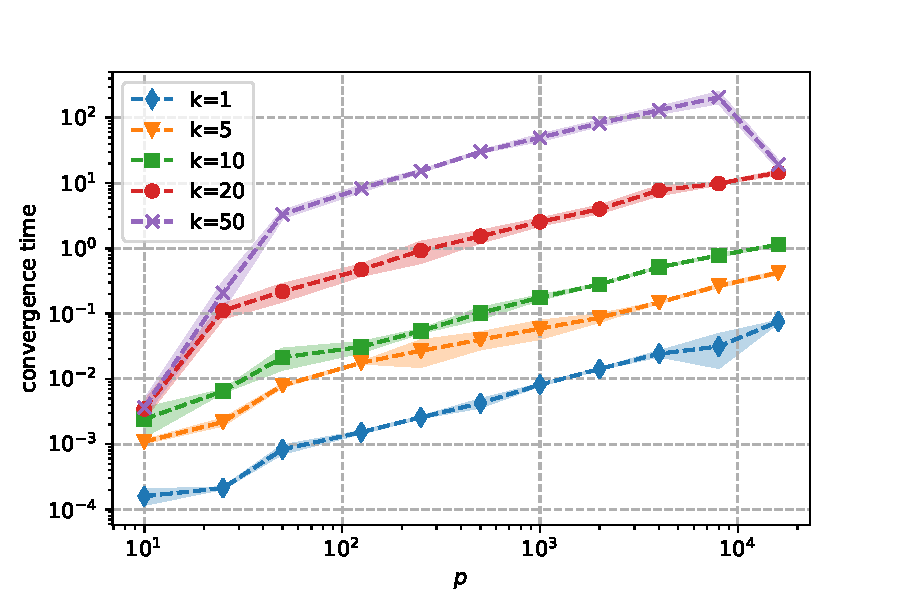
\includegraphics[width=0.8\linewidth, height=0.5\linewidth]{figures/low_rank_times.pdf}
    \caption{
        Convergence times of the low-rank coordinate ascent algorithm~\ref{alg:low_rank_coordinate_ascent}
        as a function of $p$ and $k$.
        It confirms the theoretical $\cO(n_{\text{iters}} \cdot p \cdot k^3)$ rate.
        In practice,
        the algorithm converges much faster to an appropriate solution when using a larger tolerance threshold.
        See Appendix~\ref{sec:coordinate_ascent_data} for details regarding the random data generation.
    }
    \label{fig:low_rank_times}
\end{figure}

This scheme is summarized in Algorithm~\ref{alg:low_rank_coordinate_ascent}.
It uses at most $\cO\left( p \cdot k \right)$ memory ($F$ never has to be fully computed as it's a diagonal)
and the time complexity is $\cO\left( n_\text{iters} \cdot p \cdot k^2 \right)$, as stated above.
However, numerical instabilities led us to perform some experiments in $\cO\left( n_\text{iters} \cdot p \cdot k^3 \right)$.
Figure~\ref{fig:low_rank_times} shows the convergence time for Algorithm~\ref{alg:low_rank_coordinate_ascent} as
a function of $p$ and $k$.

\subsection{Efficient low-rank sampling}\label{subsec:low_rank_sampling}

In this section, we detail briefly how to sample $\zz \sim \cN\left( \bupsilon,\, \Upsilon \right)$ once
a feasible $\bs$ is computed, and in the special case where $\cove = D + U\Lambda U^\top$.
A classical approach to sample from a multivariate normal distribution is to sample first a vector
$\tilde{\zz} \in \R^p$ from $\cN\left( 0,\, 1 \right)$,
and then pose $\zz = \bupsilon + L\tilde{\zz}$,
where $L$ is a lower Cholesky factorization of $\Upsilon$.
This uses the fact that if $\xx \sim \cN\big( \mu,\, \Sigma \big)$,
then
\begin{equation}\label{eq:affine_transformation}
    A\xx + \bb \sim \cN\big( A\bmu + \bb,\, A\Sigma A^\top \big)
\end{equation}
Note that this scheme works even if $L$ is not lower-triangular,
but only satisfies $LL^\top = \Upsilon$.

As $\Upsilon$ is a $p \times p$ matrix we may not want to store it in memory,
nor compute a Cholesky factorization (which takes $\cO\left( p^3 \right)$ steps).
We show here how to factorize $\Upsilon$ in a cheap way,
requiring only $\cO\left( k \cdot p \right)$ memory and $\cO\left( k\cdot p^2 \right)$ operations.
As shown in Section~\ref{subsec:gaussian_knockoffs}, $\Upsilon = 2S - S\cove^{-1}S$ where we note $S = \diag\bs$.
Using the low-rank structure $\cove = D + U\Lambda U^\top$,
the Sherman–Morrison–Woodbury formula (see Appendix~\ref{sec:sherman}) gives
\begin{align*}
    \cove^{-1} &= (D + UU^\top)^{-1}\\
    &= D^{-1} - D^{-1}U(I_k + U^\top D^{-1}U)^{-1}U^\top D^{-1}
\end{align*}
Note $L \in \R^{k \times k}$ the lower Cholesky factorization of
$(I_k + U^\top D^{-1}U)^{-1}$ (which can be computed efficiently if $k$ is small),
$V = SD^{-1}UL \in \R^{p \times k}$,
and $C = 2S - SD^{-1}S$.
Then the covariance reduces to
\begin{equation*}
    \Upsilon = C + VV^\top
\end{equation*}
where $C$ is diagonal and $VV^\top$ has rank at most $k$.
$C$ is not necessarily psd, which will force us to sample from a complex normal distribution.
Let $H$ be a complex square-root of $C$ (thus, potentially with imaginary numbers on the diagonal),
and $P = H^{-1}V \in \R^{p \times k}$.
Then,
\begin{equation*}
    \Upsilon = H \left( I_{p \times p} + PP^\top \right) H^\top
\end{equation*}
$\left( I_{p \times p} + PP^\top \right)$ can be factorized in the following way.
Note
\begin{equation*}
    W = \left(I_{k \times k} + \sqrt{I_{k \times k} + P^\top P}\right)^{-1} \in \R^{k \times k}
\end{equation*}
where the square-root is a $k \times k$ matrix root (which can again be computed efficiently if $k$ is small).
Then
\begin{equation*}
    I_{p \times p} + PP^\top = BB^\top
    ,\qquad
    \text{where}
    \quad
    B = I_{p \times p} + PWP^\top
\end{equation*}
Finally, we note $M = HB$ and we have that $\Upsilon = MM^\top$.
$B$ is $p \times p$ but we never have to fully evaluate it;
instead only $W$ and $P$ can be stored and matrix multiplications are then at most $p \times k$.

$M$ is a complex matrix so we cannot directly use the property~\ref{eq:affine_transformation}.
But if $\cX \sim \cN(\0,\, I)$ and $\cY = i\cX$,
then $\operatorname{Im}\left( M\cY \right) \sim \cN(\0,\, MM^\top = \Upsilon)$.
Using this scheme, with $p = 15\,000$ and $k = 100$ we can draw $n = 5\,000$ samples in $\approx 4$ seconds,
while the naive method not taking into account the low rank approximation would need $\approx 180$ seconds.
In comparison sampling $5000 \times 15\,000$ numbers from $\cN(0, 1)$ takes $\approx 2$ seconds.
